%Dokumentklasse
\documentclass[a4paper,12pt]{scrreprt}
\usepackage[left= 2.5cm,right = 2cm, bottom = 4 cm]{geometry}
%\usepackage[onehalfspacing]{setspace}
% ============= Packages =============

% Dokumentinformationen
\usepackage[
	pdftitle={Titel der Abschlussarbeit},
	pdfsubject={},
	pdfauthor={Euer Name},
	pdfkeywords={},	
	%Links nicht einrahmen
	hidelinks
]{hyperref}


% Standard Packages
\usepackage[utf8]{inputenc}
\usepackage[ngerman]{babel}
\usepackage[T1]{fontenc}
\usepackage{graphicx, subfig}
\graphicspath{{img/}}
\usepackage{fancyhdr}
\usepackage{lmodern}
\usepackage{xcolor}
\usepackage{minted}
\usepackage{framed}

\usepackage{listings}

\usepackage{wrapfig}

% zusätzliche Schriftzeichen der American Mathematical Society
\usepackage{amsfonts}
\usepackage{amsmath}

%nicht einrücken nach Absatz
%\setlength{\parindent}{0pt}


% ============= Kopf- und Fußzeile =============
\pagestyle{fancy}
%
\lhead{}
\chead{}
\rhead{\slshape \leftmark}
%%
\lfoot{}
\cfoot{\thepage}
\rfoot{}
%%
\renewcommand{\headrulewidth}{0.4pt}
\renewcommand{\footrulewidth}{0pt}

% ============= Abkürzungsverzeichnis =============
\usepackage[acronym]{glossaries}
\makeglossaries
\newacronym{RL}{RL}{Reinforcement Learning}
\newacronym{DRL}{DRL}{Deep Reinforcement Learning}
\newacronym{DNN}{DNN}{Deep Neural Network}
\newacronym{DQN}{DQN}{Deep Q-Network}
\newacronym{ML}{ML}{Machine Learning}
\newacronym{MLP}{MLP}{Multilayer Perceptron}
\newacronym{CNN}{CNN}{Convolutional Neural Network}
\newacronym{MDP}{MDP}{Markov Decision Process}
\newacronym{ABM}{ABM}{Agent-Based Modelling}
\newacronym{VFH}{VFH}{Vector Field Histogram}
\newacronym{APF}{APF}{Artificial Potential Field}
\newacronym{RRT}{RRT}{Rapidly-exploring Random Tree}
\newacronym{EAPF}{EAPF}{Evolutionary Artificial Potential Field}
\newacronym{DFID}{DFID}{Depth-First Iterative Deepening}

% ============= Package Einstellungen & Sonstiges ============= 
%Besondere Trennungen
\hyphenation{De-zi-mal-tren-nung}

%Neue Absätze
\setlength{\parindent}{0pt}
\KOMAoptions{parskip=half}

%Code Farbe
\definecolor{aliceblue}{rgb}{0.94, 0.97, 1.0}

% ============= Dokumentbeginn =============

\begin{document}
%Seiten ohne Kopf- und Fußzeile sowie Seitenzahl
\pagestyle{empty}

\begin{center}
\begin{tabular}{p{\textwidth}}


\begin{center}

\includegraphics[scale=1]{img/logo.jpg}  
\quad

\includegraphics[scale=0.4]{img/unilogo.png}
\end{center}


\\

\begin{center}
\LARGE{\textsc{
Informaticup 2021 \\
SPE\_ED\\
}}
\end{center}

\\


\begin{center}
\large{Universität Augsburg}
\end{center}

\\

\begin{center}
\textbf{\Large{Abschlussbericht}}
\end{center}


\begin{center}
vorgelegt von
\end{center}

\begin{center}
\large{\textbf{Julius Brandl}} \\
\large{\textbf{Nicolas Breinl}} \\
\large{\textbf{Maximilian Demmler}} \\
\large{\textbf{Lukas Hartmann}} \\
\end{center}

\begin{center}
\large{im Januar 2021}
\end{center}

\end{tabular}
\end{center}


\addsec{Abstract}
\label{cha:abstrakt}

\emph{Im vorliegenden Bericht wird die Entwicklung einer Software beschrieben, die das Multiplayer-Spiel Spe\_ed selbstständig spielt. Nach der Evaluierung von klassischen Robotik- und RL-Ansätzen wird ein Minimax-Ansatz aus der Spieltheorie vorgestellt und für das Problem weiterentwickelt. Der Multi-Minimax-Algorithmus erlaubt die Anwendung auf mehr als zwei Spieler und eine Voronoi-Heuristik wird als passende Evaluierungsfunktion für Spe\_ed eingeführt. Der Aufbau der Python-Software wird vorgestellt und verschiedene Versionen gegeneinander evaluiert. Dabei zeigt SW-RG-V-Multi-Minimax Vorteile gegenüber anderen Ansätzen. Auswertungen gegen andere Teams auf dem Live-Server ergeben Gewinnraten von mehr als 80\%.}




% Beendet eine Seite und erzwingt auf den nachfolgenden Seiten die Ausgabe aller Gleitobjekte (z.B. Abbildungen), die bislang definiert, aber noch nicht ausgegeben wurden. Dieser Befehl fügt, falls nötig, eine leere Seite ein, sodaß die nächste Seite nach den Gleitobjekten eine ungerade Seitennummer hat. 
\cleardoubleoddpage

% pagestyle für gesamtes Dokument aktivieren
\pagestyle{fancy}

%Inhaltsverzeichnis
\tableofcontents

%Verzeichnis aller Bilder
\listoffigures

%Verzeichnis aller Tabellen
\listoftables

\chapter{Einleitung}
\label{cha:Einleitung}

In den folgenden Abschnitten werden wir Ihnen den Verlauf unserer Teilnahme am \textit{InformatiCup 2021} präsentieren und einen Überblick über die weiteren Kapitel bieten. Die gesamte Ausarbeitung ist bewusst in einem lockeren Ton und mit direkter Ansprache formuliert, um den Lesefluss angenehmer zu gestalten.

In den ersten Tagen nach dem Start des Wettbewerbs haben wir uns mit der Aufgabenstellung vertraut gemacht und besondere Herausforderungen erarbeitet. Dabei ist uns aufgefallen, dass \textit{Spe\_ed} im Prinzip eine Erweiterung des Spielmodus \textit{Light Cycles} aus dem Arcade-Spiel \textit{Tron}\footnote{https://de.wikipedia.org/wiki/Tron\_(Computerspiel)} ist. Wesentliche Unterschiede zu Light Cycles sind:
\begin{itemize}
    \item Die Spielfeldgröße ist variabel
    \item Die Anzahl der Spieler ist variabel
    \item Die Zeit für einen Zug ist beschränkt und variabel
    \item Spieler können unterschiedliche Geschwindigkeiten besitzen
    \item Alle 6 Runden entstehen Lücken in den Spuren schneller Spieler
\end{itemize}
Diese Erweiterungen stellen zugleich auch die besonders herausfordernden Eigenschaften des Spiels dar. Dennoch bieten bereits existierende algorithmische Ansätze für Light Cycles eine gute Grundlage für Spe\_ed. In den Kapiteln \ref{cha:Ansaetze} und \ref{cha:voronoi} gehen wir unter anderem genauer darauf ein, von welchen Light Cycles -Ansätzen wir uns inspirieren lassen haben und wie wir mit den genannten Herausforderungen umgehen.

Nachdem wir uns ein gutes Bild von der Aufgabenstellung gemacht hatten, haben wir durch altbewährtes Brainstorming und Mindmapping versucht, ein möglichst breites Spektrum an Lösungsansätzen zu erarbeiten. Dabei haben wir die drei - auf der InformatiCup-Website\footnote{https://informaticup.github.io/challenges/spe-ed} angerissenen - übergeordneten Lösungsansätze \textit{Spieltheorie}, \textit{künstliche Intelligenz} und \textit{Planungsheuristik} als Ausgangspunkt verwendet. Folgende Kernideen haben wir letztendlich als am vielversprechendsten erachtet:
\begin{itemize}
    \item Trajektorienplanung
    \item \acrfull{RL}
    \item Tiefensuche
\end{itemize}
Diese Ansätze haben wir in der initialen Projektphase parallel näher untersucht und Prototypen implementiert. In Kapitel \ref{cha:Ansaetze} bieten wir einen Überblick über verwandte Arbeiten zu den jeweiligen Ansätzen, heben Schwächen und Stärken hervor und begründen die Entscheidung die Tiefensuche als finalen Ansatz zu wählen. Da Spe\_ed nur über eine Webschnittstelle gespielt werden kann, haben wir zu diesem Zeitpunkt außerdem entschieden, das Spiel nachzuimplementieren. Zum einen ermöglicht das unsere Ansätze gezielt und effizient offline testen zu können. Zum anderen ist es für \acrshort{RL} und Tiefensuche grundlegend notwendig Zugriff auf ein vom Algorithmus kontrollierbares Modell von Spe\_ed zu haben. Kapitel \ref{cha:software} beschäftigt sich näher mit unserer Vorgehensweise bei der Modellierung von Spe\_ed.

Den größten Abschnitt des Wettbewerbs haben wir verwendet, um die Tiefensuche zu implementieren und durch Erweiterungen und Optimierungen zu ergänzen. Im Speziellen haben wir einen Multi-Minimax-Algorithmus entworfen, der die sogenannte Voronoi-Heuristik als Hauptevaluationskriterium verwendet. In Kapitel \ref{cha:voronoi} wird der Algorithmus im Detail vorgestellt.

Letztendlich hatten wir gegen Ende des Wettbewerbs mehrere Varianten des Algorithmus mit unterschiedlichen Erweiterungen implementiert. Um eine finale Abgabe zu bestimmen, haben wir ausgewählte Varianten in unserem Modell gegeneinander antreten lassen und die Spiele ausgewertet. Zusätzlich haben wir erfolgreiche Varianten auch auf dem Online-Server des InformatiCup getestet. In Kapitel \ref{cha:Ergebnisse} präsentieren wir die Ergebnisse dieser Auswertungen.

Alles in allem können wir behaupten, dass unsere Lösung gute Resultate erzielt. Trotzdem ist uns natürlich bewusst, dass unser Algorithmus - wie vermutlich jeder Algorithmus mit derzeitiger Rechenleistung - nicht in allen Spielpositionen die allgemeingültig beste Aktion wählt. Daher betrachten wir unseren Ansatz in Kapitel \ref{cha:Diskussion} in einem kritischen Licht und bieten Ideen für zukünftige Forschungen.



\chapter{Ansätze und Related Work}
\label{cha:Ansaetze}
Wir haben \textit{Trajektorienplanung}, \textit{\acrlong{RL}} und \textit{Spieltheorie} als vielversprechendste Ansätze für Spe\_ed erachtet und genauer unter die Lupe genommen. Die folgenden Unterkapitel fassen unsere Erkenntnisse zur Anwendbarkeit der jeweiligen Ansätze und Untersuchungen verwandter Arbeiten zusammen.

\section{Trajektorienplanung}

Spe\_ed kann wie folgt betrachtet werden: F\"ur einen Agenten m\"ussen Steuerbefehle erzeugt werden, die zu einer Reihe von Wegpunkten mit Geschwindigkeiten - also einer Trajektorie - f\"uhren. Der Pfad soll zudem Kollisionen vermeiden. Diese Betrachtungsweise f\"uhrt zum Ansatz, das Problem mithilfe von Trajektiorienplanung aus der klassischen Robotik zu l\"osen. Einige der prominentesten Vertreter dieser Algorithmen sind \acrfull{VFH} \cite{Borenstein.}, \acrfull{RRT}\cite{S.Karaman.2011}, Voronoi-Diagramm \cite{Garrido.2006}, und \acrfull{APF} \cite{Raja.2012}. Wir haben uns entschieden, den letztgenannten Ansatz zu testen, da dieser die Umgebung in einer f\"ur Spe\_ed passend erscheinenden Weise darstellt. Beim \acrshort{APF} wird die Umgebung als ein Feld von Potenzialen modelliert, bspw. indem Hindernisse ein hohes abstoßendes Potenzial erhalten. Der Agent bestimmt dann zur Pfadplanung den Weg des steilsten Abstiegs (\"uber den Gradient). Passend f\"ur Spe\_ed, da große Freifl\"achen bevorzugt und Gegner gemieden werden. Zudem kann der Algorithmus mit evolution\"aren Ans\"atzen kombiniert werden, woraus bspw. das \acrfull{EAPF} entsteht. \cite{Raja.2012} 

Der L\"osungsansatz alleine \"uber Trajektorienplanung bringt allerdings einige Probleme mit sich. Das Bedeutendste ist, dass Trajektorienplanung alleine keine Strategie finden kann. Vielmehr implementiert es eine zuf\"allige oder vom Entwickler erdachte Strategie, z.B. \glqq halte m\"oglichst großen Abstand zu Hindernissen\grqq. Das ist auch dadurch bedingt, dass in der klassischen Robotik meist ein Ziel wie \glqq fahre diesen Punkt an\grqq{} oder \glqq halte genau diesen Abstand zum Fahrer vor dir\grqq{} vorgegeben ist. In unserer Aufgabe ist das Ziel zu abstrakt (\glqq gewinne das Spiel\grqq{}/\glqq Überlebe länger als die anderen\grqq{}). Besonders das evaluierte \acrshort{APF} schafft es mit der typischen Parameterkonfiguration nicht Gegner abzuschneiden oder den Platz nahe an W\"anden effizient zu nutzen.\footnote{W\"ande erhalten normalerweise ein abstoßendens Potenzial, allerdings ist es an sich sinnvoll, nahe heranzufahren.} Aus den genannten Gr\"unden wurde dieser als alleiniger wieder verworfen, allerdings taucht das Voronoi-Diagramm im finalen Ansatz auf.

\section{\acrlong{RL}}
% kurze Einleitung
In den letzten Jahren haben \acrshort{RL}-Algorithmen beeindruckende Fortschritte gezeigt. Mittlerweile übertreffen sie beispielsweise menschliche Spitzenleistungen in Atari-Spielen, Schach, Shogi, Go und Dota 2 \cite{Mnih.19.12.2013, Silver.2018b, OpenAI.2019}. Daher ist es nur naheliegend, \acrshort{RL} auch für den diesjährigen InformatiCup als Ansatz in Betracht zu ziehen.

% Kurze RL-Def
\acrshort{RL} beschäftigt sich mit der Fragestellung, wie Software-\textit{Agenten} lernen können, eine bestimmte Aufgabe in einer bestimmten \textit{Umgebung} zu meistern \cite{Sutton.1998}. Im Bezug auf den diesjährigen InformatiCup ist die Umgebung das Spiel Spe\_ed, der Agent ein Spieler und die Aufgabe zu gewinnen. Es gibt allerdings noch ein paar Eigenheiten von Spe\_ed, die die Anwendung von \acrshort{RL} erschweren: (1) Die Spielfeldgröße ist variabel, (2) Die Anzahl der Gegenspieler ist variabel, (3) Die \textit{Policy} (Verhaltensweise) der Gegenspieler ist unbekannt.

% MDP
Der Lernprozess bei \acrshort{RL} wird typischerweise durch den \acrfull{MDP} beschrieben: Der Agent führt in jedem Zeitschritt $t$ eine Aktion $a_t$ aus, die den Zustand $s_t$ der Umgebung verändert. Nachdem $a_t$ ausgeführt wurde, empfängt der Agent von der Umgebung einen neuen Zustand $s_{t+1}$ und eine Belohnung $r_{t+1}$. Die \textit{Policy} $\pi$ eines Agenten legt die Aktion fest, die er in einem bestimmten Zustand ausführt. Genauer ist $\pi(a|s)$ die Wahrscheinlichkeit, dass der Agent die Aktion $a$ im Zustand $s$ wählt. Ziel eines \acrshort{RL}-Algorithmus ist, eine Policy zu erlernen, die die akkumulierten, in Zukunft erwarteten Belohnungen - kurz: \textit{Return} - maximiert. \cite{Sutton.1998}

% Zustandsraum
Um \acrshort{RL} auf Spe\_ed anzuwenden, müssen wir also erst einmal den Zustandsraum modellieren. Dabei kommen einem bereits die Variabilität der Spielfeldgröße und der Spieleranzahl in die Quere. Denn an sich könnte man einen Spielzustand vollständig beschreiben, wenn man den Zustandsraum mit folgenden Informationen ausstattet:
\begin{itemize}
	\item Die Belegung der Felder auf dem Spielfeld (mit möglichen Zahlencodierungen -1 bis \# Spieler)
	\item Die Positionen aktiver Spieler
	\item Die Bewegungsrichtungen aktiver Spieler
	\item Die Geschwindigkeiten aktiver Spieler
	\item Einen Rundenzähler
\end{itemize}
\acrshort{RL}-Algorithmen fordern allerdings eine Zustandsdarstellung mit einer festen Anzahl an Zustandsattributen. Zur Lösung dieses Problems gibt es zwei Ansätze: (1) Die maximal mögliche Zustandsgröße wählen und kleinere Zustände mit bestimmten \textit{Padding-Werten} auf die maximale Größe erweitern. (2) Nur einen Ausschnitt der Umgebung mit fester Größe betrachten (z.B. nur x Felder in jede Richtung um den Agenten herum und nur die nächsten y anderen Spieler betrachten). Dabei können beide Ansätze miteinander kombiniert werden. In jedem Fall steht jedoch fest, dass der Zustandsraum sehr groß ist - ein Spielfeld der Größe 50x50 mit 5 Spielern hätte mit den oben aufgelisteten Informationen modelliert \[Höhe*Breite+4*Spieler+1=50*50+4*5+1=2.521\] Zustandsattribute. Um den Ansatz nicht von vorn herein zu verkomplizieren, haben wir zunächst eine kleine, feste Spielfeldgröße und nur einen Gegenspieler als Umgebung angenommen.

% Self-Play
Bevor wir uns nun mit den eigentlichen \acrshort{RL}-Algorithmen beschäftigen können, muss allerdings noch eine weitere Frage geklärt werden: Gegen wen spielt unser Agent eigentlich während des Trainings? Man kann den Agent zwar auf einem leeren Spielfeld trainieren, allerdings würde dieser wohl lediglich lernen, alle Felder so langsam wie möglich auszufüllen, um die unausweichliche Eliminierung so lange wie möglich hinauszuzögern.\footnote{Der Agent erhält die Belohnung 1 für einen Siegeszug, -1 bei Eliminierung und sonst 0.} Es kommt auch nicht infrage den Agent gegen einen eigens entwickelten Gegenspieler spielen zu lassen, denn unser Agent würde nur lernen, gegen diesen einen Gegner zu gewinnen. Der derzeit beste Ansatz für solch ein Problem ist das sogenannte \textit{Self-Play}, wie es beispielsweise \textit{Google} und \textit{DeepMind} bei \textit{AlphaZero} \cite{Silver.2018b} und \textit{OpenAI Five} \cite{OpenAI.2019} verwenden. Hierbei tritt der Agent immer wieder gegen sich selbst an und lernt somit automatisch gegen Gegenspieler mit unterschiedlicher Policy zu spielen. Um \acrshort{RL}-Agenten letztendlich in Spe\_ed trainieren zu können, haben wir unser Spe\_ed-Modell in ein \textit{Gym-Environment} \cite{Brockman.2016} eingekapselt und die Schnittstellen vektorisiert, um Self-Play zu ermöglichen.

% Q-Learning
Der wohl bekannteste \acrshort{RL}-Ansatz ist das 1989 von Chris Watkins vorgestellte \textit{Q-Learning} \cite{Watkins.1992}. Q-Learning lernt die optimale \textit{Aktionswert-Funktion $q_*$} mit Q zu approximieren. Q wird dabei tabellarisch dargestellt, weshalb der Ansatz nur auf Umgebungen mit diskreter Zustands- und Aktionsdarstellung anwendbar ist. Das ist vorerst kein Problem, da beides bei Spe\_ed diskret dargestellt werden kann. Was hingegen problematisch ist, ist die Größe des Zustandsraumes. Bereits auf einem 3x3 Spielfeld mit 2 Spielern gibt es $4^{3*3}=262.144$ mögliche Belegungen des Spielfelds.\footnote{Die Basis der Berechnung ergibt sich durch $\# Spieler + 2$, da dies der Anzahl der möglichen Belegungen eines Feldes entspricht: -1 (Kollision), 0 (Frei), x (Spieler x)} Das bedeutet, dass alleine durch ein 3x3 Spielfeld - von Informationen über Spielerpositionen etc. abgesehen - eine Q-Tabelle mit $262.144$ Einträgen benötigt wird. Man kann die Q-Tabelle zwar dynamisch gestalten und den Zustandsraum durch Symmetrieüberlegungen etwas verkleinern, allerdings explodiert der Zustandsraum trotzdem spätestens bei Spielfeldern größer als 5x5 zu nicht umsetzbaren Größen. Wir konnten Q-Learning-Agenten zwar erfolgreich auf einem 3x3 Spielfeld trainieren, allerdings können solch kleine Spielfelder auch durch Tiefensuche in sehr kurzer Zeit optimal gelöst werden. Daher ist ein tabellarischer Ansatz ungeeignet.

% DRL - DQN
2013 haben Mnih et al. einen neuen Meilenstein im Bereich des \acrshort{RL} gesetzt, indem Sie \acrfullpl{DNN} als Funktionsapproximatoren zur Approximation der Q-Funktion beim Q-Learning verwenden \cite{Mnih.19.12.2013, Mnih.2015}. Das dabei entstandene \acrfull{DQN} haben Minh et al. erfolgreich verwendet, um Atari 2600 Spiele zu spielen. Im Gegensatz zum tabellarischen Q-Learning können \acrshortpl{DQN} kontinuierliche Zustandsdarstellungen als Eingang verwenden. Das reduziert die Größe der Zustandsdarstellung bei Spe\_ed drastisch - ein 3x3 Spielfeld kann nun unabhängig von der Anzahl der möglichen Belegung eines Feldes mit $3*3=9$ Zustandsattributen beschrieben werden. Des Weiteren können \acrshortpl{DQN} Verallgemeinerungen über Spielzustände lernen. Das hat den Vorteil, dass sie nicht jeden konkreten Spielzustand gesehen haben müssen, um ihn bewerten zu können.

% MLP vs CNN
Statt dem standardmäßigen \acrfull{MLP} haben Mnih et al. ein \acrfull{CNN} als Netzwerkarchitektur verwendet, da sich \acrshortpl{CNN} besonders gut für die Verarbeitung von Bildern (bzw. \textit{Spiel-Frames}) eignen. Bei Spe\_ed reicht eine rein bildliche Darstellung des Spielfelds allerdings nicht zur Beschreibung des Zustands aus - es fehlen die Informationen über Spielerpositionen, -geschwindigkeiten und -bewegungsrichtungen. Daher haben wir eine reine \acrshort{MLP}-Architektur und eine Architektur mit getrennten \acrshort{CNN} und \acrshort{MLP}-Eingangslayer, die in tieferen Layern zusammengeführt werden, auf Spe\_ed getestet. Leider haben beide Architekturen jedoch auch nach längerer Trainingszeit keine guten Ergebnisse geliefert.

% Begründung für Entscheidung gegen RL
Zu diesem Zeitpunkt haben wir uns dafür entschieden, den \acrshort{RL}-Ansatz nicht weiter zu verfolgen und uns auf die Tiefensuche zu konzentrieren. Folgende Probleme vermuten wir als Hauptgründe für das Scheitern: (1) Der Zustandsraum ist selbst kontinuierlich betrachtet sehr groß - deutlich größer als beispielsweise beim Schach; (2) aufgrund unserer begrenzten Ressourcen können wir die \acrshort{DQN}-Architektur nicht tief/groß genug wählen und das \acrshort{DQN} nicht lange genug trainieren; (3) Self-Play kann den Trainingsverlauf destabilisieren und benötigt für erfolgreiche Ergebnisse besonders viel Trainingszeit \cite{Bai.22.06.2020}.


\section{Spieltheorie}
\label{cha:spieltheorie}

Nat\"urlich darf bei den Ans\"atzen zur L\"osung eines Spiels auf keinen Fall die Spieltheorie vergessen werden. Laut Wikipedia ist die Spieltheorie \glqq eine mathematische Theorie, in der Entscheidungssituationen modelliert werden, in denen mehrere Beteiligte miteinander interagieren. Sie versucht dabei unter anderem, das rationale Entscheidungsverhalten in sozialen Konfliktsituationen davon abzuleiten\grqq{} \cite{wikipedia_spieltheorie} - klingt sehr passend.

Bei Spe\_ed handelt es sich um ein Konstantsummenspiel (spieltheoretisch \"aquivalent zum Nullsummenspiel) mit perfekter Information. Wir kennen also das gesamte bisherige Spielgeschehen und wenn wir gewinnen, verliert der Gegner. Ein simpler Gedanke, eine Strategie f\"ur ein derartiges Spiel zu entwerfen ist, alle m\"oglichen Verl\"aufe aufzuz\"ahlen und den Gewinner am Ende zu bestimmen. Somit k\"onnten wir in jeder Situation den Zug w\"ahlen, bei dem wir am Ende gewinnen.\footnote{Vorausgesetzt, die Gegner spielen nicht perfekt. Wenn alle Spieler perfekt spielen, gewinnt der mit der besten Startposition.} 

Da Spe\_ed aus spieltheoretischer Sicht damit dem Schach sehr \"ahnlich ist, erwies sich eine Analyse der dort verwendeten Techniken als sinnvoll. Die meisten Algorithmen f\"ur Schach verwenden diese Suchb\"aume bzw. Spielb\"aume in verschiedenen Formen und Kombinationen. F\"ur uns erschien der Minimax-Algorithmus gut anwendbar.

Dabei wird ein Suchbaum aufgebaut, der alternierend Ebenen enth\"ahlt in denen der eigene Spieler bzw. der gegnerische Spieler am Zug ist. Der eigene Spieler versucht seinen Gewinn zu maximieren, daher sind dies die maximierenden Levels. Die Gegner versuchen den Gewinn vom eigenen Spieler zu minimieren, dies sind daher die minimierenden Levels. \cite{Shannon.1950, Campbell.1983}

Versuchen wir einen Suchbaum nun am Beispiel eines 4x4 Feldes mit zwei Spielern aufzustellen. Für den ersten Zug hat jeder Spieler 5 M\"oglichkeiten seine Aktion zu w\"ahlen,\footnote{Praktisch  können es auch weniger sein, in der ersten Runde bspw. f\"uhrt slow\_down zu Geschwindigkeit 0. Hier soll es allerdings um eine Worst-Case Absch\"atzung gehen.} das ergibt $5^{2} = 25$ Spielsituationen nach Runde eins. Nun kann wieder jeder Agent aus 5 Aktionen w\"ahlen, dadurch kommen  $5^{2} = 25$ M\"oglichkeiten zustande, in Runde zwei zu agieren. Insgesamt k\"onnen also auf 25 Situationen 25 M\"oglichkeiten gebaut werden, f\"ur Runde zwei ergeben sich dadurch $(5^{2})^{2} = 625$ Situationen. In Runde drei stehen nun 625 Situationen zur Verf\"ugung, wieder gibt es 25 Kombinationen darauf zu agieren, also $625 \cdot 25 = 15625$. In Runde vier gibt es bereits 390.625 Zust\"ande, in Runde f\"unf 9.765.625, in Runde $n$: $(5^{2})^{n}$. Bei einem Spiel auf 4x4 mit zwei Spielern kann es maximal $16 / 2 - 1 = 7$ Runden geben, daf\"ur gibt es 6.103.515.625 Spielverl\"aufe. Der Zustandsraum ist also (v.a. f\"ur gr\"ossere Felder) zu gewaltig, um alle Verl"aufe aufzuz\"ahlen. Allerdings erweisen sich einige Pfade relativ schnell als unbrauchbar wegen eines zu schlechten Ergebnisses in diesen Pfaden. Um diese Pfade auszuschließen und damit eine Beschleunigung zu erreichen, ist ein vielgenutztes Verfahren das Alpha-Beta-Pruning \cite{Knuth.1975}. Hierzu werden zwei Werte \textit{Alpha} und \textit{Beta} eingeführt, die den minimalen Wert, den der maximierende Spieler bzw. den maximalen Wert, den der minimierende Spieler erreichen kann, darstellen. Sobald in einem Teilbaum klar ist, dass dieser kein besseres Ergebnis (bzw. schlechteres bei gegnerischem Spieler) erreichen kann, wird dieser ausgeschlossen. Dies ist in Abb. \ref{fig:alphabeta} dargestellt.


\begin{figure}[h]
    \centering
    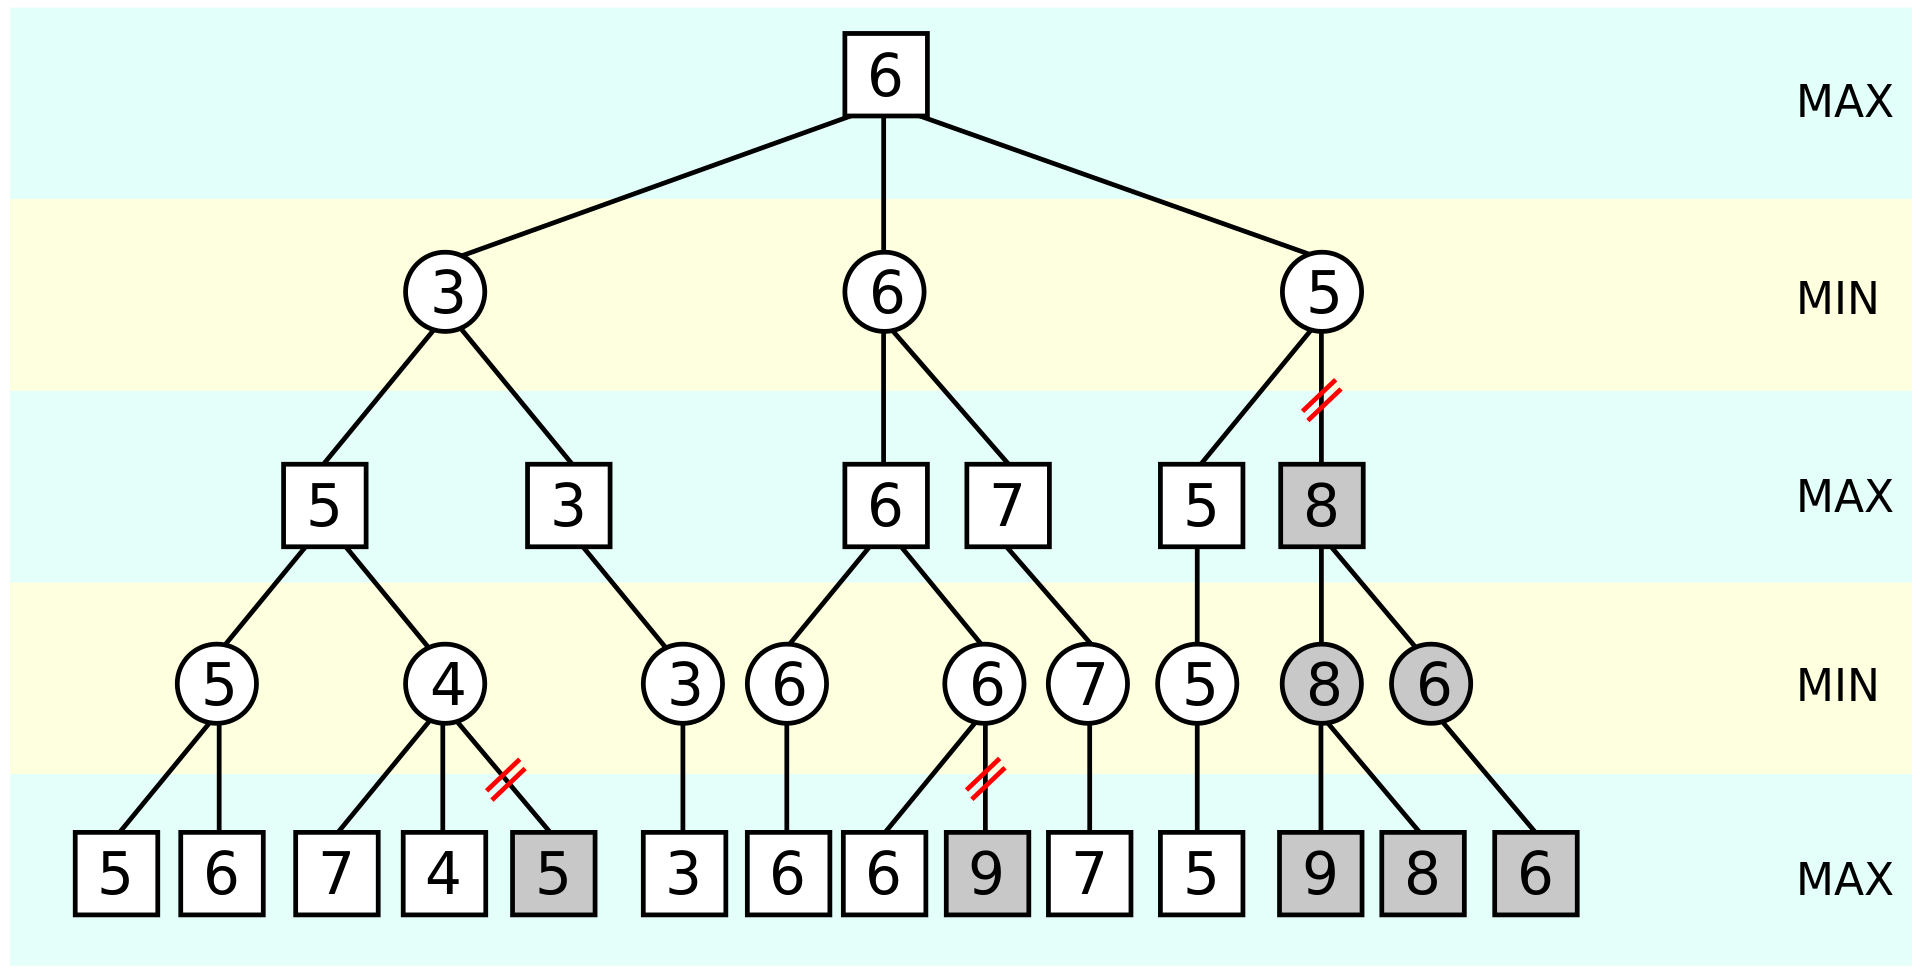
\includegraphics[width=\textwidth]{img/AB_pruning.svg.png}
    \caption[Minimax mit Alpha-Beta-Pruning]{Minimax mit Alpha-Beta-Pruning. Graue Pfade werden nicht beachtet, da sie auf jeden Fall nichts mehr am Ergebnis verbessern. Abbildung aus \cite{wikipedia_alpha_beta} entnommen.}
    \label{fig:alphabeta}
\end{figure}

Trotz der Reduktion der Pfade durch Alpha-Beta-Pruning ist es meist nicht möglich, alle Pfade bis auf die unterste Tiefe zu berechnen. Der Suchbaum kann stattdessen nur bis zu einer gewissen Tiefe durchsucht werden. Allerdings steht der Sieger in dieser Tiefe oftmals noch nicht fest - wie also zwischen den Aktionen w\"ahlen? An dieser Stelle kommt nun die Bewertungsfunktion ins Spiel. So wird bspw. mittels einer Heuristik die Situation bewertet. F\"ur Spe\_ed hat sich Voronoi als eine passende Bewertungsheuristik ergeben.

Die meisten Arbeiten beschäftigen sich mit Zwei-Spieler-Problemen. Bei Spe\_ed handelt es sich jedoch um ein Multi-Player-Problem. Perez und Oommen stellen in \cite{Perez.2019} eine einfache Erweiterung des Minimax-Algorithmus auf mehrere Spieler vor.




\chapter{Voronoi-Basierter Multi-Minimax Algorithmus}
\label{cha:voronoi}

In diesem Kapitel stellen wir den Multi-Minimax-Algorithmus und eine auf Voronoi-Diagrammen basierende Situationsbewertung vor. Zudem beschreiben wir zusätzliche Erweiterungen, die den Algorithmus bestmöglich auf Spe\_ed anpassen.

\section{Multi-Minimax}

Es existieren bereits mehrere Ansätze um Minimax auf Multiplayer-Spiele zu erweitern: \textit{Paranoid \cite{Sturtevant.2006}, Max\textsuperscript{n} \cite{.1986}}, \textit{Best Reply Search} \cite{Schadd.2011} und Multi-Minimax \cite{Perez.2019}. Multi-Minimax wurde in der Arbeit von Perez und Oommen gegen die oben genannten Algorithmen am Spiel \textit{Light Cycles} getestet. Der vorgestellte Algorithmus erzielte dabei sowohl bei 4-Spieler-Situationen als auch bei 6-Spieler-Situatioen bei über 20.000 getesteten Spielen die besten Ergebnisse. Darüber hinaus bietet er uns den Vorteil, dass er bereits für simultane Spiele, also Spiele mit gleichzeitigen Zügen ausgelegt ist. Der Algorithmus läuft in \textit{O(nb\textsuperscript{d})} für n = Spieleranzahl, b = \textit{branchingfactor}\footnote{Anzahl der Aktionen} und d = Anzahl der Spielrunden \cite{Perez.2019}. Daher verwenden wir Multi-Minimax auch für unseren Lösungsansatz.

Beim Multi-Minimax-Algorithmus tritt der maximierende Spieler immer isoliert gegen einen minimierenden Spieler an. Nachdem jeder Gegenspieler isoliert betrachtet wurde, wird die eigene Aktion basierend auf dem besten Gegenspieler gewählt. Dabei verwendet der Algorithmus Alpha-Beta Pruning und die in Kapitel \ref{cha:spieltheorie} beschriebene Minimax-Routine. In Abbildung \ref{fig:multiminimax} ist ein Entscheidungsbaum der Tiefe drei abgebildet.

Die Heuristik die Perez und Oommen für die Situationsbewertung verwenden, ist simpel. Falls der Gegenspieler nicht mehr aktiv ist und der eigene Spieler noch mögliche Züge hat, die nicht zum Tod führen, wird die Situation mit dem best-möglichen Wert unendlich bewertet. Andernfalls wird die Situation mit der erreichten Suchtiefe bewertet. Diese Heuristik ist sehr praktisch für kleine Spielfelder (12x12 im Fall von Perez und Oommen), da sie wenig Rechenaufwand benötigt und somit fast alle möglichen Züge berechnet werden können. In unserem Fall ist sie aber nicht ideal, weil das Spielfeld bei Spe\_ed bis 80x80 groß werden kann. Dafür ist eine Heuristik notwendig, die Informationen über das ganze Spielfeld liefert und einschätzt, wie gut ein Spieler momentan ist - unabhängig davon, ob er in x Zügen sterben würde. Deshalb haben wir die in Kapitel \ref{cha:voronoi} vorgestellte Voronoi-Heuristik gewählt.

\begin{figure}[ht]
    \centering
    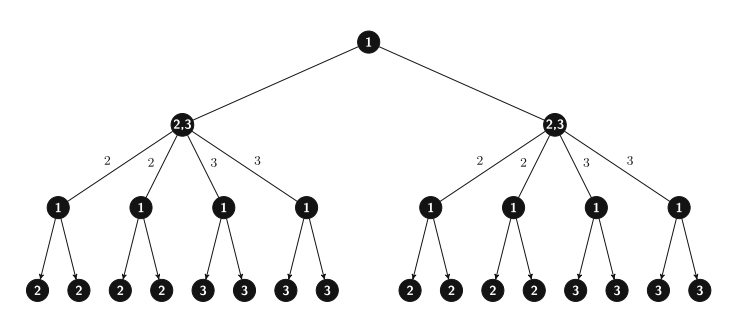
\includegraphics[width=1\textwidth]{img/multiminimax.PNG}
    \caption[Multi-Minimax]{Multi-Minimax Repräsentation für 3 Spieler und branching-Faktor 2. Die Knoten geben an, welcher Spieler als nächstes an der Reihe ist, die Kanten repräsentieren die Aktionen. Grafik aus \textit{Multi-Minimax: A New AI Paradigm for Simultaneously-Played Multi-player Games \cite{Perez.2019}}}
	\label{fig:multiminimax}
\end{figure}

\section{Voronoi-Heuristik}
\label{cha:voronoi_sec}

Ein Voronoi-Diagramm (vgl. Abbildung \ref{fig:voronoi}) gibt an, welche Felder des Spielfeldes von welchem Spieler zuerst erreicht werden können. Felder die gleichzeitig erreicht werden können werden als \textit{battlefront} bezeichnet (Lila Felder in Abbildung \ref{fig:voronoi}). Die Idee zu diesem Ansatz kam erstmals während der \textit{Google AI Challenge}\footnote{https://de.wikipedia.org/wiki/AI Challenge} auf \cite{AndySloane.2010}. Die Voronoi-Heuristik bewertet nun eine Spielsituation basierend auf der Differenz der zuerst erreichbaren Felder des eigenen Agenten und des jeweiligen Min-Agenten. Da wir bei Spe\_ed im Gegensatz zur \textit{Google AI Challenge} verschiedene Geschwindigkeiten haben, müssten wir das Voronoi-Diagramm unter Betrachtung der derzeitigen Geschwindigkeiten und möglicher Geschwindigkeitsänderungen aller Spieler berechnen. Wir haben diese Erweiterung implementiert und evaluiert, sind aber zu dem Schluss gekommen, dass der gewonnene Vorteil im Vergleich zum stark erhöhten Rechenaufwand zu gering ist. Eine Erweiterung und Verbesserung der Voronoi-Heuristik für das klassische \textit{Tron}-Game ist die \textit{Tree-of-Chambers}-Heuristik \cite{AndySloane.2010, Kang.2012}. Diese ist jedoch für Spielfelder mit vielen einzelnen Lücken ungeeignet \cite{Kang.2012}. Da bei Spe\_ed ein zerklüftetes Spielfeld durch das regelmäßige Entstehen von Lücken häufiger vorkommt, haben wir uns schlussendlich für die Voronoi-Heuristik ohne Tree-of-Chambers-Erweiterung entschieden.

\begin{figure}[ht]
    \centering
    \includegraphics[width=0.4\textwidth]{img/voronoi.PNG}
    \caption[Voronoi-Diagramm]{Voronoi-Diagramm für vier Spieler auf einem 50x50 Feld. Spielerpositionen in Schwarz dargestellt; Voronoi-Regionen der jeweiligen Spieler in Grün, Rot, Gelb und Türkis; Battlefronts in Lila.}
	\label{fig:voronoi}
\end{figure}

\section{Erweiterungen}
\label{cha:Erweiterungen}

Die beiden vorgestellten Grundkonzepte \textit{Multi-Minimax} und \textit{Voronoi-Heuristik} haben wir durch einige Erweiterungen angepasst, um sie bestmöglich für Spe\_ed verwenden zu können. Diese Erweiterungen werden im Folgenden vorgestellt.

\subsection{Vorsortierung der Aktionen}

Beim Alpha-Beta-Pruning können mehr Pfade eliminiert werden, wenn die Aktionen für die Mulit-Minimax-Suche nach ihrer Ausführungswahrscheinlichkeit vorsortiert werden. Durch Beobachtungen hat sich folgende Reihenfolge als optimal ergeben:
\begin{enumerate}
    \item change\_nothing
    \item turn\_left
    \item turn\_right
    \item speed\_up
    \item slow\_down
\end{enumerate}

\subsection{Endgame-Erkennung}

Wir überprüfen zu Beginn des Algorithmus ob wir uns in einem \textit{Endgame} befinden. Wir befinden uns in einem \textit{Endgame}, sobald wir keinen Gegner mehr direkt erreichen können, ohne dabei über eine Mauer zu springen. Ein Endgame wird wieder aufgelöst, sobald wir in den Bereich eines Gegners springen oder ein Gegner in unseren Bereich springt. Sobald wir uns in einem Endgame befinden, simulieren wir nur die eigenen Züge und ignorieren das Verhalten der Gegner. Dies erlaubt uns, eine größere Tiefe für den Multi-Minimax Algorithmus zu erreichen und somit in einer gewinnenden Position unseren verfügbaren Bereich nahezu perfekt auszufüllen und in einer verlierenden Position mehr Möglichkeiten zu evaluieren, um aus unserem Bereich heraus zuspringen und somit das Endgame aufzulösen.  

\subsection{Wall-Hugging}

Wir fügen, wie es Andy Sloane in \cite{AndySloane.2010} beschreibt, einen \textit{territory-bonus} hinzu. Dabei werden offene Felder aus der eigenen Voronoi-Region höher gewichtet als Felder mit mehr Wänden. Dies führt automatisch dazu, das unser Agent im Falle eines Voronoi-Gleichstands eher an Wänden entlang fährt und somit seinen eigenen Platz weniger verbaut. 

\subsection{Reduktion der betrachteten Gegner}

Da bei sechs Spielern der Berechnungsaufwand für Multi-Minimax im Vergleich zu weniger Spielern stark erhöht ist, schränken wir die betrachteten Gegenspieler ein. Wir ermitteln gleichzeitig zur Endgame Erkennung die Gegenspieler, deren Voronoi-Regionen auf unsere treffen. Wir schließen Gegenspieler aus, die wir nicht erreichen können, weil sie eine Wand von uns trennt oder ein weiterer Spieler dazwischen positioniert ist. Wir gehen davon aus, dass das Verhalten dieser Spieler für uns vorerst nicht relevant ist. Wären wir zum Beispiel in Abbildung \ref{fig:voronoi} der Spieler mit der grünen Voronoi-Region, würden wir den Spieler mit der gelben Voronoi-Region vorerst nicht betrachten, da diese Voronoi-Regionen nicht aufeinandertreffen.

\subsection{Einschränkung der eigenen Geschwindigkeit}

Wir haben beobachtet, dass unser Agent bei höheren Geschwindigkeiten teilweise schlechte Entscheidungen trifft. Die Suchtiefe, die wir im Falle von knappen \textit{Deadlines} (unter 8 Sekunden) erreichen, reicht nicht aus, um bei hohen Geschwindigkeiten Kollisionen zu vermeiden. Deshalb haben wir uns entschieden, die maximale Geschwindigkeit unseres Agenten auf drei zu beschränken. Diese Geschwindigkeit ermöglicht es uns trotzdem noch die regelmäßig entstehende Lücke geschickt zu nutzen. Wir heben diese Einschränkung auf, sobald wir uns im Endgame befinden. Dadurch kann unser Agent mehr Möglichkeiten berechnen, im Falle eines verlierenden Endgames aus dem eigenen Bereich zu springen und eine verlierende Position zu einer gewinnenden zu drehen. 

\subsection{\acrlong{DFID}}

Für die Berechnung der nächsten Aktion wird in Spe\_ed jeweils eine Zugzeit vorgegeben. Somit müssten wir bei der Tiefensuche die maximale Tiefe für den Suchbaum genau so wählen, dass alle Äste in der vorgegebenen Zeit abgearbeitet werden. Dies ist offensichtlich sehr fehleranfällig. Wählen wir hingegen einen Breitensuche-Ansatz, wird schnell viel Speicherplatz benötigt. Einen Kompromiss zwischen beiden Varianten bietet \acrfull{DFID}. Dabei wird die Tiefensuche auf eine maximale Tiefe begrenzt, sobald diese Tiefe abgeschlossen ist, wird die maximale Tiefe erhöht und der Baum erneut durchlaufen. Das verursacht zwar, dass die oberen Bereiche des Baumes (unnötig) mehrfach berechnet werden, da der Baum nach unten allerdings exponentiell größer wird, ist dies verschmerzbar. \cite{Korf.1985}

Somit wird die gewählte Aktion mit steigender Suchtiefe inkrementell verbessert. Zum einen garantieren wir damit, dass unser Algorithmus auch bei kurzen Zugzeiten eine passende Aktion findet. Zum anderen nutzt der Algorithmus die volle Zugzeit aus und sucht bei längeren Zeiten nach Lösungen in tieferen Suchebenen. Wir starten die Berechnung der auszuführenden Aktion in einem Subprozess, während im Hauptprozess die aktuelle Serverzeit abgefragt und die verfügbare Zeit berechnet wird. Sobald die Zeit abgelaufen ist, terminiert der Hauptprozess das \acrshort{DFID} und erhält über eine zwischen den Prozessen geteilte Variable die auszuführende Aktion. Zur Kommunikation mit dem Server verwenden wir Python's \textit{asyncio}\footnote{https://docs.python.org/3/library/asyncio.html}.


\subsection{Multiprocessing}
Zur Verbesserung der Berechnungsgeschwindigkeit wird \textit{Multiprocessing} verwendet. Dabei wird die \acrshort{DFID} Methode genutzt, jedoch werden die Berechnungen für die verschiedene Tiefen gleichzeitig gestartet. Dabei werden bis zu 6 Tiefen gleichzeitig berechnet, aber nicht mehr, als der Prozessor verschiedene Threads zur Verfügung stellt. Die auszuführende Aktion wird bei jedem Abschluss einer neuen Tiefe aktualisiert. Nach Ende der vorgegebenen Berechnungszeit werden alle Prozesse gestoppt und die berechnete Aktion zurückgegeben.

Außerdem wird anfangs ein Prozess erstellt, der MultiMiniMax mit Tiefe 2 und ohne Voronoi berechnet. Auf dieses Ergebnis kann zurückgegriffen werden, falls nur eine sehr kurze Berechnungszeit vorhanden ist. Dadurch kann, falls es die Spielsituation erlaubt, immer eine Aktion gefunden werden, mit der der Agent im nächsten Schritt nicht stirbt. Da die Berechnungsdauer bei größeren Tiefen allerdings exponentiell steigt, steigert das Multiprocessing die erreichten Tiefen in der Praxis nicht und führt bei der Ausführung unter verschiedenen Betriebssystemen eventuell zu Zeitverzögerungen beim Erstellen der Prozesse. Daher verwenden wir den Ansatz nicht für unsere finale Abgabe.

\subsection{Cython}
Damit die Performance noch weiter verbessert werden kann, wird \textit{Cython}\footnote{https://cython.org/} verwendet. Dadurch kann der Python-Code in schnelleren C-Code kompiliert werden. Zur einfacheren Wart- und Erweiterbarkeit wird aber darauf verzichtet statisches Typing, also die explizite Angabe des Datentyps einer Variable, zu nutzen. Somit müssen nach Erweiterung des Python-Codes keine weiteren Änderungen erfolgen, sondern die geänderten Dateien müssen lediglich neu gebaut werden. Durch das Kompilieren des Voronoi-Moduls konnte so eine Geschwindigkeitssteigerung von ca. 8\% erreicht werden.

\subsection{Sliding Window}
Um die Komplexität des Problems zu verkleinern, wird nur ein Teil des Spielfelds betrachtet. Der Ausschnitt (Sliding Window), der betrachtet wird, wandert dabei mit der aktuellen Position unseres Agenten. Als Kompromiss zwischen Komplexität und einer trotzdem ausreichenden Spielbeschreibung hat sich eine Größe von 20 Feldern in jede Richtung als guter Wert für die Größe des Fensters herausgestellt. Hierdurch werden nur Gegner betrachtet, die sich in der Nähe unseres Agenten befinden und ihn in nächster Zeit beeinflussen können. Gegner außerhalb dieses Sliding-Window werden ignoriert, wodurch eine weitere Komplexitätsminimierung stattfindet.

Für den Fall, dass sich kein Gegner in unserem Fenster befindet, wird das Fenster so weit erweitert, sodass sich mindestens ein anderer Spieler in dem Fenster befindet. Darüber hinaus wird das Fenster um einen festen Offset erweitert.

Die Erweiterung wird umgesetzt, indem die vom Server erhaltene Spielbeschreibung bereits vor der Überführung in unser Modell passend zugeschnitten wird. Somit sind keine weiteren Änderungen an den verwendeten Algorithmen notwendig und die Erweiterung ist leicht austauschbar.

\subsection{Kamikaze}
Bisher erhält der Agent in der Situationsbewertung keinen Bonus dafür, Gegner zu eliminieren. Falls der Agent der eigenen Eliminierung im nächsten Schritt nicht mehr entkommen kann führt er somit eine zufällige Aktion aus. Die Erweiterung \textit{Kamikaze} sorgt dafür, dass er in solchen Fällen, falls möglich, eine Aktion wählt, die einen Gegner eliminiert (und somit eventuell zu einem Unentschieden statt einer Niederlage führt). Wir verallgemeinern den Bonus für die Eliminierung von Gegenspielern bewusst nicht auf alle Spielpositionen, um zu verhindern, dass der Agent die Eliminierung von Gegnern über bessere Strategien hinweg wählt.


\chapter{Software}
\label{cha:software}

Wie bereits in Kapitel \ref{cha:Einleitung} erwähnt, war die Nachimplementierung/Simulation von Spe\_ed unser erster Implementierungsschritt. Da die eingesetzten Modellierungstechniken- und Frameworks einen maßgeblichen Einfluss auf die gesamte Architektur haben, stellen wir unser Vorgehen bei der Modellierung in diesem Kapitel genauer vor. Außerdem gehen wir auf die Punkte Software-Architektur, Software-Testing und Wartbarkeit/Erweiterbarkeit ein.

Zunächst noch ein paar allgemeinere Angaben zur Software: Wir haben uns für die Programmiersprache \textit{Python} entschieden, da sie ein breites Spektrum an bewährten Werkzeugen für Modellierung, \acrshort{RL} und Datenanalyse bietet. Wir verwenden die Python-Version 3.7, unsere Implementierungen sind streng nach den Coding Conventions des \textit{PEP 8 Style Guide}\footnote{https://www.python.org/dev/peps/pep-0008/} formatiert und \textit{Core}-Klassen und -Funktionen sind durchgehend mit \textit{Docstrings}\footnote{https://www.python.org/dev/peps/pep-0257/} dokumentiert.

\section{Architektur und Modellierung}
\label{sec:modellierung}

Die Software-Architektur unseres Projektes ist in die Software-Pakete \textit{Core}, \textit{Evaluation} und \textit{Scripts} geteilt. \textit{Core} stellt den funktionalen Kern unseres Projekts dar. Es enthält das Spe\_ed-Modell und die implementierten Spieler-Algorithmen (\textit{Agents}). \textit{Evaluation} beinhaltet unsere Auswertungssoftware und \textit{Scripts} enthält beispielsweise Skripte zur Online-Ausführung unserer Agenten. Abbildung \ref{fig:komponentendiagramm} zeigt den beschriebenen Aufbau und die Abhänigkeitshirarchie zwischen den Software-Paketen.

\begin{figure}[ht]
    \centering
    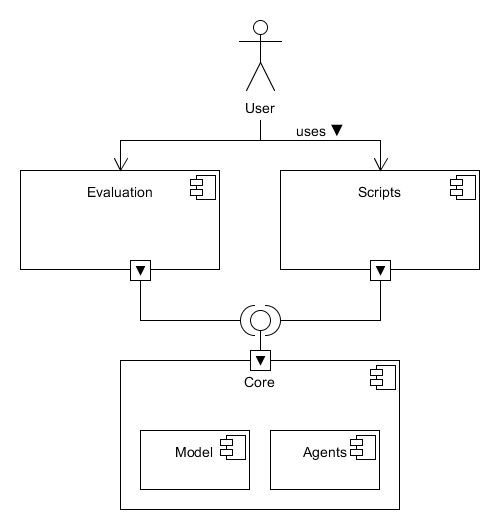
\includegraphics[width=0.7\textwidth]{img/architecture.png}
    \caption{Komponentendiagramm unseres Projekts}
	\label{fig:komponentendiagramm}
\end{figure}

Unsere grundlegende Idee hinter der Modellierung von Spe\_ed ist, dass das Modell wie eine Black-Box verwendet werden kann, deren Schnittstellen mit denen des originalen Spiels übereinstimmen. Die Input- und Output-Formate des Modells entsprechen daher exakt den JSON-Formaten des originalen Spiels. Somit kann eine entwickelte Spieler-Software ohne Änderungen sowohl im Modell als auch im Original ausgeführt werden.

Als Modellierungsansatz haben wir uns für \acrfull{ABM} entschieden. \acrshort{ABM} verfolgt einen \textit{Bottom-Up}-Ansatz zur Modellierung von Simulationen. Das bedeutet, dass der Ablauf der Simulation nicht zentral von ’oben’ herab gesteuert wird, sondern dass die autonomen Individuen der Simulation (genannt \textit{Agenten}) den Simulationsverlauf durch ihr jeweiliges Verhalten von ’unten’ aus bestimmen. Die zentralen Komponenten von \acrshort{ABM} sind (1) mehrere Agenten und (2) die Umgebung, in der sich die Agenten befinden. \acrshort{ABM} eignet sich besonders gut zur Modellierung und Simulation von Spe\_ed, da Spe\_ed ein Multi-Agenten-System ist, in dem die Agenten ein eigenes - nicht zentral vorgegebenes - Verhalten besitzen. Bei Simulationen wird zudem zwischen \textit{ereignisbasierten} (auch \textit{asynchronen}) und \textit{zeitorientierten} (auch \textit{synchronen}) Modellen unterschieden. Bei Spe\_ed handelt es sich um ein System in dem alle Agenten in festen Zeitschritten eine Entscheidung treffen. Deshalb ist es sinnvoll ein zeitorientiertes Modell zu wählen. \cite{Bernhardt.2007, Macal.2009}

Um unsere Software möglichst effizient, wartbar und leicht verständlich zu gestalten nutzen wir ein Simulationsframework. Auf Basis der oben genannten Kriterien haben wir \textit{Mesa} \cite{Masad.2015} als Framework für die Implementierung unseres Spe\_ed-Modells gewählt. Mesa wurde 2015 als erstes \acrshort{ABM}-Framework für Python veröffentlicht. Es ist \textit{open-source} und orientiert sich an anderen \acrshort{ABM}-Tools und -Frameworks, wie \textit{NetLogo} \cite{Wilensky.2004}, \textit{Repast} \cite{North.2013} und \textit{MASON} \cite{Luke.2005}. Mesa besitzt zudem einen leichtgewichtigen und somit effizienten Framework-Kern. Das Framework ordnet seine Komponenten drei verschiedenen Modulen zu: Modellierung, Visualisierung und Analyse. Wir beschäftigen uns im Folgenden zwar lediglich mit der Modellierung, allerdings ist es nennenswert, dass wir unser Modell durch die Nutzung von Mesa ohne beachtlichen Mehraufwand web-basiert visualisieren und analysieren können.

Das Modellierungsmodul von Mesa implementiert den \acrshort{ABM}-Ansatz. Es besteht aus den Basisklassen \textit{Model}, \textit{Agent}, \textit{Scheduler} und \textit{Space}. Die \textit{Model}-Klasse enthält Modellparameter und steuert (startet, stoppt, etc.) den Ablauf einer Simulation. In der \textit{Agent}-Klasse wird definiert, welche Prozesse ein Agent bei seiner Aktivierung durchläuft - die Aktivierung eines Agenten entspricht bei uns der Ausführung eines Zuges. Der \textit{Scheduler} verwaltet die Simulationszeit. Er kennt alle Agenten und aktiviert diese in jedem Zeitschritt. Die \textit{Space}-Klasse beschreibt den Raum, in dem sich die Agenten befinden. Mesa bietet von Haus aus mehrere Unterklassen der \textit{Scheduler}- und \textit{Space}-Klassen an. In unserem Anwendungsfall wird der \textit{SimultaneousActivation}-Scheduler und der \textit{MultiGrid}-Space verwendet.

\begin{figure}[ht]
    \centering
    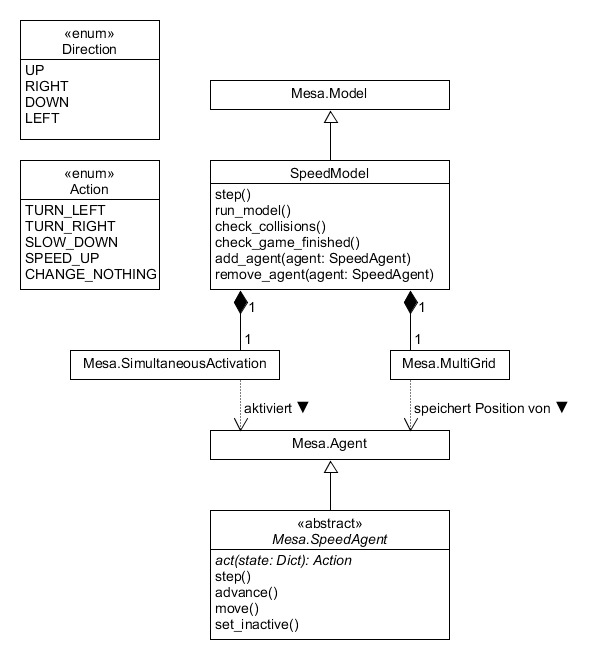
\includegraphics[width=0.8\textwidth]{img/model.png}
    \caption{Vereinfachtes Klassendiagramm der Modell-Architektur}
	\label{fig:model}
\end{figure}

Abbildung \ref{fig:model} zeigt ein vereinfachtes Klassendiagramm unserer Modell-Architektur. Klassen die Bestandteil von Mesa sind, sind mit dem Präfix \textit{Mesa.} versehen. Im Mittelpunkt stehen die Klassen \textit{SpeedModel} und \textit{SpeedAgent}. Diese sind eigens implementiert und beschreiben die Funktionsweise des Modells. Die  \textit{SpeedAgent}-Klasse ist abstrakt und besitzt die abstrakte Methode \textit{act(state)}. Hier haben wir die oben genannte Black-Box-Schnittstelle platziert. Der Übergabeparameter \textit{state} entspricht dem JSON-Format eines Spielzustands von Spe\_ed und der Rückgabewert ist die Aktion für die sich der Spieler entschieden hat. Um einen bestimmten Agenten zu entwerfen muss also lediglich eine Klasse erstellt werden, die von  \textit{SpeedAgent} erbt und die  \textit{act}-Methode implementiert. Diese Struktur macht unsere Software leicht um neue Agenten erweiterbar.

Um die einfache Verwendung unserer Software zu demonstrieren, zeigen wir in Abbildung \ref{fig:model_code} wie beispielsweise ein Spiel mit einem \textit{RandomAgent} (Agent der zufällige Aktionen trifft) und einem \textit{MulitMinimaxAgent} (siehe Kapitel \ref{cha:voronoi}) gestartet wird. Das Beispiel verdeutlicht außerdem, dass Modellparameter wie die Spielfeldgröße variabel und leicht einstellbar sind.

\begin{figure}[ht]
    \centering
    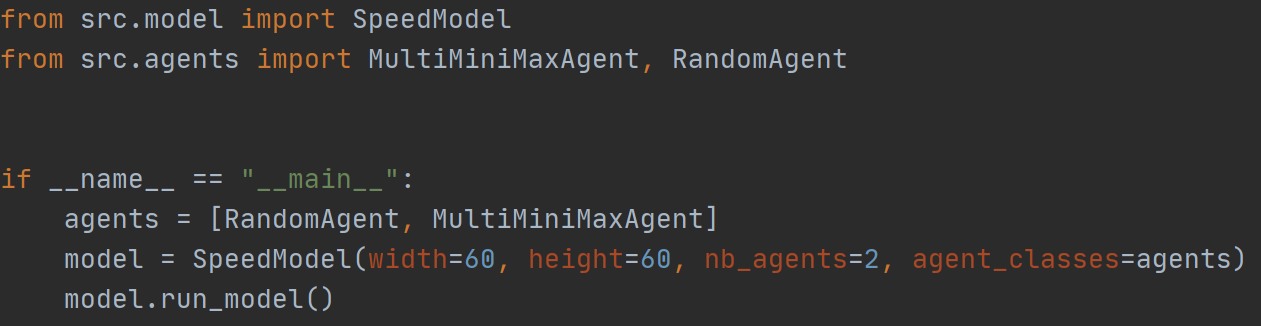
\includegraphics[width=0.9\textwidth]{img/model_code.PNG}
    \caption{Code-Beispiel zur Erstellung und Ausführung des Modells}
	\label{fig:model_code}
\end{figure}


\section{Software-Testing}
\label{sec:testing}

Das Schreiben von Software-Tests war für uns aus zwei Gründen besonders wichtig. Zum einen mussten wir sicher gehen können, dass unser Modell mit dem originalen Spiel übereinstimmt. Zum anderen war es wichtig, dass wir Erweiterungen und Optimierungen an den algorithmischen Ansätzen leicht validieren können. Die Tests sind - wie bei \textit{Unit Tests} in Python standardmäßig vorgesehen - in Software-Paketen namens \textit{tests}, auf gleicher Ebene wie das zu testende Modul, eingebettet.

Beim Testen des Modells kommt uns erneut die Black-Box-Eigenschaft zugute. Wir verwenden JSON-Dateien von gespeicherten Original-Spielen und gleichen in den Tests die Spielzustände zu jedem Zeitschritt mit denen unseres Modells ab. Dabei laden wir zuerst den initialen Spielzustand eines gespeicherten Spiels in das Modell, extrahieren dann die Aktionen der Spieler/Agenten zu den jeweiligen Zeitschritten und simulieren diese Aktionen dann auf unserem Modell. Wenn das Modell alle 58 gespeicherten Spiele korrekt simuliert, ist der Modell-Test bestanden. Auf diese Weise erhalten wir deutlich umfangreichere Tests, als durch manuelles Erstellen von Test-Spielzuständen möglich wäre.

Die implementierten Agenten und deren Algorithmen (Multi-Minimax, Voronoi, etc), werden mit Unit-Tests abgedeckt. Dabei testen wir, insbesondere ob die Agenten bei ausreichender Suchtiefe in verschiedenen Spielsituationen den besten Zug finden. Zu allen übrigen \textit{Core}-Softwaremodulen (wie z.B. \textit{utils}) haben wir ebenfalls Unit Tests geschrieben. Wie in Abbildung \ref{fig:coverage} zu sehen erreichen wir insgesamt eine Testabdeckung von 84\% für das \textit{Core}-Softwaremodul.

\begin{figure}[ht]
    \centering
    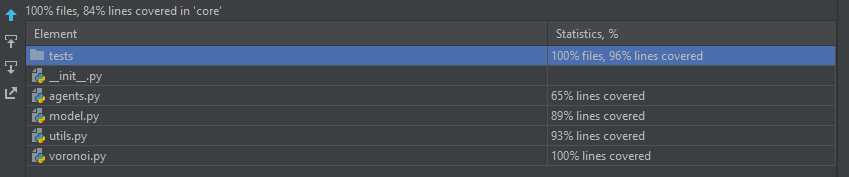
\includegraphics[width=0.9\textwidth]{img/coverage.PNG}
    \caption{Testabdeckung für das \textit{Core}-Softwaremodul}
	\label{fig:coverage}
\end{figure}

\chapter{Ergebnisse}
\label{cha:Ergebnisse}

Um unsere Software auszuwerten haben wir sie auf dem Live-Server und mit Hilfe unseres Modells getestet. In den folgenden Unterkapiteln stellen wir die resultierenden Ergebnisse vor und interpretieren ihre Bedeutung.

\section{Live-Server}

Wir haben über den Verlauf des Wettbewerbs verschiedene Versionen unserer Lösung auf dem Live-Server antreten lassen. Zum einen um unsere eigene Lösung zu evaluieren und zum anderen um Informationen über das Spiel und über die Gegenspieler zu sammeln. Abbildung \ref{tab:Spiel_Parameter} zeigt die Ergebnisse der gesammelten Informationen über die Spielfeldbreite, Spielfeldhöhe und die verfügbare Zeit pro Zug. In zwei beobachteten Spielen hatte das Spielfeld eine Größe von 80x80. Da wir weder für die Breite noch für die Höhe des Spielfelds jemals einen Wert > 80 beobachtet haben, können wir annehmen, dass es sich bei 80x80 um die maximale Spielfeldgröße handelt. Das kleinste von uns beobachtete Spielfeld hatte eine Größe von 43x41. Dadurch können wir approximiert von einem kleinsten Spielfeld der Größe 41x41 ausgehen. Die von uns ermittelte durchschnittliche Zugzeit beträgt \textasciitilde10 Sekunden. Unter Berücksichtigung der Latenz nehmen wir an, dass die Zugzeiten Zufallszahlen zwischen \textasciitilde5 und \textasciitilde15 Sekunden sind.

% Spiel-Parameter
\begin{table}[t]
	\begin{tabular}{|c|c|c|c|c|}
		\hline 
		Metrik & Höhe & Breite & Zugzeit \\
		\hline\hline
		Minimum & 41 & 41 & 3,26s \\
		\hline 
		Maximum & 80 & 80 & 14,94s \\
		\hline 
		Mittelwert & 60.13 & 61 & 9,66s \\
		\hline
	\end{tabular}
	\centering
	\caption[Auswertung der Spiel-Parameter]{Auswertung der Spiel-Parameter}
	\label{tab:Spiel_Parameter}
\end{table}

Da unserer Lösungsansatz sowohl mit variablen Spielfeldgrößen als auch mit variablen Zugzeiten umgehen kann, haben diese Erkenntnisse keinen direkten Einfluss auf unseren Lösungsansatz. Jedoch konnten wir die gesammelten Informationen vor allem für eigene Offline-Auswertungen verwenden, um den Live-Server so gut wie möglich nachzubilden und unsere Ansätze mit verschiedenen Parametern darauf zu testen.

Wir haben über die letzten beiden Wochen des Wettbewerbes auf dem zur Verfügung gestellten Live-Server eine in 120 Spielen eine Gewinnrate von 82\% erzielt. Fragwürdig ist jedoch wie aussagekräftig dieser Wert ist, da wir jeweils verschiedene Versionen unserer Lösung getestet haben, und wir bei vielen der Spielen vermuten, dass es sich bei unseren Gegnern vermehrt um Bots der Wettbewerbsveranstalter und nicht um andere Teams gehandelt hat.  


\section{Offline-Versionsauswertung}

%Versuchsaufbau (Spielfeldgröße etc + Verweis auf Data Mining, Agenten)
Um aus den verschiedenen Versionen unserer Agenten eine finale Version für die Abgabe zu bestimmen haben wir ausgewählte Versionen im Modell gegeneinander spielen lassen. Im Folgenden werden die verwendeten Versionen beschrieben, wobei sich die Erweiterungen auf Kapitel \ref{cha:Erweiterungen} beziehen:
\begin{itemize}
    \item \textbf{Multi-Minimax}: Multi-Minimax-Algorithmus \cite{Perez.2019} ohne weitere Erweiterungen
    \item \textbf{V-Multi-Minimax}: Multi-Minimax mit Voronoi-basierter Positionsauswertung und den Erweiterungen \textit{Cython}, \textit{Wall-Hugging}, \textit{Vorsortierung der Aktionen}, \textit{Endgame Erkennung}, \textit{Einschränkung der eigenen Geschwindigkeit}, \textit{\acrshort{DFID}} und \textit{Kamikaze}
    \item \textbf{RG-V-Multi-Minimax}: V-Multi-Minimax mit der Erweiterung \textit{Reduktion der betrachteten Gegner}
     \item \textbf{SW-RG-V-Multi-Minimax V1}: RG-V-Multi-Minimax mit der Erweiterung \textit{Sliding Window} mit Fenstergröße 40 und Offset 5
    \item \textbf{SW-RG-V-Multi-Minimax V2}: RG-V-Multi-Minimax mit der Erweiterung \textit{Sliding Window} mit Fenstergröße 30 und Offset 3
\end{itemize}

% Fair start evaluation
Damit die Erkenntnisse der Auswertungen im Modell möglichst gut auf die Live-Instanz von Spe\_ed übertragbar sind, haben wir die Auswertungsparameter an den Ergebnissen aus Tabelle \ref{tab:Spiel_Parameter} orientiert. Dabei muss bei den beobachteten Zugzeiten noch die mögliche Latenz berücksichtigt werden. Tabelle \ref{tab:Auswertungsparameter} zeigt die gewählten Auswertungsparameter. Wir verwenden ein Spielfeld der Größe 60x60 und wählen eine Zugzeit zufällig zwischen 5 und 15 Sekunden. Da Spiele auf Feldern dieser Größe häufig sehr lange dauern (im Schnitt ca. 6 Stunden), ist es leider nicht möglich eine hohe Anzahl an Versuchswiederholungen durchzuführen. Spe\_ed ist allerdings ein stark initialisierungsabhängiges Spiel - Spieler mit schlechten Startpositionen haben geringere Gewinnchancen. Um die Aussagekraft der Ergebnisse bei wenigen Versuchswiederholungen trotzdem hoch zu halten, initialisieren wir die Positionen nicht zufällig. Stattdessen generieren wir für alle 5 Agenten für jeweils 5 Spiele Positionen und rotieren diese innerhalb der 5 Spiele durch, sodass jeder Agent einmal von jeder Startposition aus startet. Agent 1 erhält also in Spiel 2 die Position die Agent 2 in Spiel 1 hatte und Agent 2 die alte Position von Agent 3 usw. Nach 5 gespielten Partien werden neue Positionen generiert. Somit ist die Initialisierung fair und die Auswertungen sind bereits bei geringer Anzahl an Versuchswiederholungen aussagekräftig.


% Auswertungsparameter
\begin{table}[t]
	\begin{tabular}{|c|c|c|c|c|}
		\hline 
		Höhe & Breite & \# Spieler & Zugzeit &  Versuchswiederholungen \\
		\hline\hline
		60 & 60 & 5 & rand(5, 15) & 60 \\
		\hline 
	\end{tabular}
	\centering
	\caption[Auswertungsparameter]{Auswertungsparameter}
	\label{tab:Auswertungsparameter}
\end{table}

% Ergebnisse & Interpretation & Fazit
Tabelle \ref{tab:Versionen} zeigt die Ergebnisse der Auswertung. Dargestellt sind die Gewinnraten der einzelnen Agenten sowie deren durchschnittliche Platzierung. Die Platzierung ergibt sich über die Ausscheidungsreihenfolge, wobei der Gewinner Platz 1 erhält.\footnote{Bei Ausscheidung in der gleichen Runde wird eine Platzierung geteilt - beide erhalten die bessere Platzierung.} Es ist eindeutig erkennbar, dass sich die Voronoi-basierte Situationsauswertung auszahlt, da alle Voronoi-basierten Algorithmen den reinen Multi-Minimax-Algorithmus weit übertreffen. Die Erweiterungen \textit{Sliding Window}- und \textit{Reduktion der betrachteten Gegner} zeigen zudem wiederum eine Verbesserung im Vergleich zum V-Multi-Minimax-Agent. Das liegt daran, dass sie es schaffen die Komplexität der Situationsauswertung zu reduzieren, um eine höhere Suchtiefe zu erreichen, ohne relevante Informationen über die Umgebung zu vernachlässigen. Die beiden SW-RG-V-Multi-Minimax-Varianten schneiden am besten ab. Grund dafür ist vermutlich, dass sie im Schnitt tiefere Suchebenen als RG-V-Multi-Minimax erreichen und daher auch bei geringen Zugzeiten gut durchdachte Aktionen wählen. Interessanterweise erreicht Variante 2 (V2) der SW-RG-V-Multi-Minimax-Agenten im Schnitt eine leicht bessere Platzierung (2,1) als Variante 2 (2,3), obwohl Variante 1 eine höhere Gewinnrate erzielt (35\% zu 28,33\%). Das lässt vermuten, dass Variante 1 noch aggressiver gespielt hat, um wenn möglich einen Sieg zu erringen. Da die Wettbewerbsveranstalter die Gewinnrate als Hauptauswertungskriterium ausgeben \footnote{https://github.com/informatiCup/InformatiCup2021/issues/15} erachten wir SW-RG-V-Multi-Minimax V2 als unseren besten Agenten und verwenden diesen in der finalen Abgabe.

% Evaluation
\begin{table}[t]
	\begin{tabular}{|c|c|c|c|c|}
		\hline 
		Algorithmus & Gewinnrate & Platzierung \\
		\hline\hline
		Multi-Minimax & 0\% & 4,22 \\
		\hline 
		V-Multi-Minimax & 11,67\% & 3,67 \\
		\hline 
		RG-V-Multi-Minimax & 25\% & 2,62 \\
		\hline
		SW-RG-V-Multi-Minimax V1 & 35\% & 2,3 \\
		\hline 
		SW-RG-V-Multi-Minimax V2 & 28,33\% & 2,1 \\
		\hline 
	\end{tabular}
	\centering
	\caption[Auswertung verschiedener Versionen]{Durchschnittswerte der Auswertung verschiedener Versionen in 60 Spielen}
	\label{tab:Versionen}
\end{table}


\chapter{Diskussion}
\label{cha:Diskussion}

Auf unseren Weg zur in Kapitel \ref{cha:voronoi} vorgestellten Lösung sind wir mit den drei Möglichkeiten Trajektorienplanung, \acrshort{RL} und Spieltheorie gestartet. Nachdem Trajektorienplanung kaum Strategie entwickeln konnte und \acrshort{RL} ebenfalls keine beachtlichen Erfolge vorweisen konnte, intensivierten wir einen Minimax-Ansatz aus der Spieltheorie - auch weil dieser in ähnlichen Spielen wie bspw. Schach verwendet wird. Der Ansatz wurde zum Multi-Minimax-Algorithmus von Perez und Oommen erweitert und wiederum durch Voronoi-Evaluierung sowie weitere Heuristiken ergänzt.

Die zugehörige Python-Software implementiert die genannten Lösungen nach dem \acrshort{ABM}-Schema. Wichtige Bestandteile der Software werden mit Tests abgedeckt. Die verschiedenen Lösungen und Erweiterungen wurden mithilfe des Modells untereinander verglichen und ausgewertet. Auswertungen am Live-Server ergaben hohe Gewinnraten (~85\%). 

In der vorliegenden Arbeit werden state-of-the-art Algorithmen aus dem Bereich Spieltheorie verwendet und für das Spiel Spe\_ed erweitert und optimiert. Der modulare und generische Code lässt sich gut erweitern. Mit der \textit{Cython}-Erweiterung wird ein Geschwindigkeitsboost erreicht, allerdings ließe sich die Geschwindigkeit (und damit die erreichte Suchtiefe) bei Verwendung einer anderen Programmiersprache vermutlich noch einmal deutlich steigern. Die Begrenzung der maximalen Geschwindigkeit des Agenten kann zudem dazu führen, dass gute Strategien ausgeschlossen werden.

Zukünftige Arbeit an dieser Problemstellung könnte die Implementierung des Voronoi-Multi-Minimax Algorithmus in \textit{C++} sein. Zudem könnten ausführliche Parameterstudien zur Fenstergröße unseres SW-RG-V-Mulit-Minimax-Algorithmus die Performance noch leicht steigern. Mit viel Rechenpower und ausreichend Zeit könnte sich zudem ein \acrshort{RL}-Ansatz lohnen und bessere Resultate erzielen. Ein Vorteil des \acrshort{RL} ist, dass die Ausführung eines trainierten Modells in der Regel schnell vonstatten geht.


% Abbildungsverzeichnis
\printglossary[type=\acronymtype, nonumberlist, title=Abkürzungsverzeichnis, toctitle=Abkürzungsverzeichnis]
%\glsaddallunused

%Literaturverzeichnis
\bibliographystyle{unsrtdin}
\bibliography{Literatur}

\end{document}
